\chapter{Prezentacja działania aplikacji}
\label{cha:prezentacja}

W tej części pracy znajduje się opis aplikacji widzianej oczami użytkownika. W rozdziale~\ref{sec:interfejsUzytkownika} został
przedstawiony interfejs graficzny użytkownika. Następnie rozdział~\ref{sec:praktyczneUzycieSystemu} prezentuje działanie aplikacji wykorzystując przykładowe dane hospitalizacji. W rozdziale tym znajduje się opis praktycznego użycia systemu dla realnych danych. Sekcja~\ref{sec:testyIntegracyjne} zawiera przykładowy test integracyjny jednej ze ścieżek poszukiwania rozwiązania.

%---------------------------------------------------------------------------

\section{Interfejs użytkownika}
\label{sec:interfejsUzytkownika}
Aplikacja ma standardowy interfejs aplikacji desktopowej napisanej w języku JAVA. Skórka aplikacji jest ustawiona na przyjazny ,,PlasticXPLookAndFeel''.

Jeden z szablonowych widoków, który chciałem zaprezentować w tej pracy to widok bazy pacjentów. Warto zaznaczyć, że wszystkie funkcjonalności, takie jak dodawanie, usuwanie, filtrowanie oraz cały widoczny układ komponentów graficznych dostarcza framework Valkyrie-RCP. Realizuje je klasa DataEditor, która jest komponentem graficznym(Widgetem), do którego wstrzykujemy DataProvider - fasadę danych dla interfejsu użytkownika, DetailForm - formę do dodawania/usuwania danych, FilterForm formę dla dodatkowego filtrowania oraz TableWidget - obiekt definiujący wyświetlaną tabelkę danych. Poniższy rysunek ilutruje widok bazy pacjetnów:

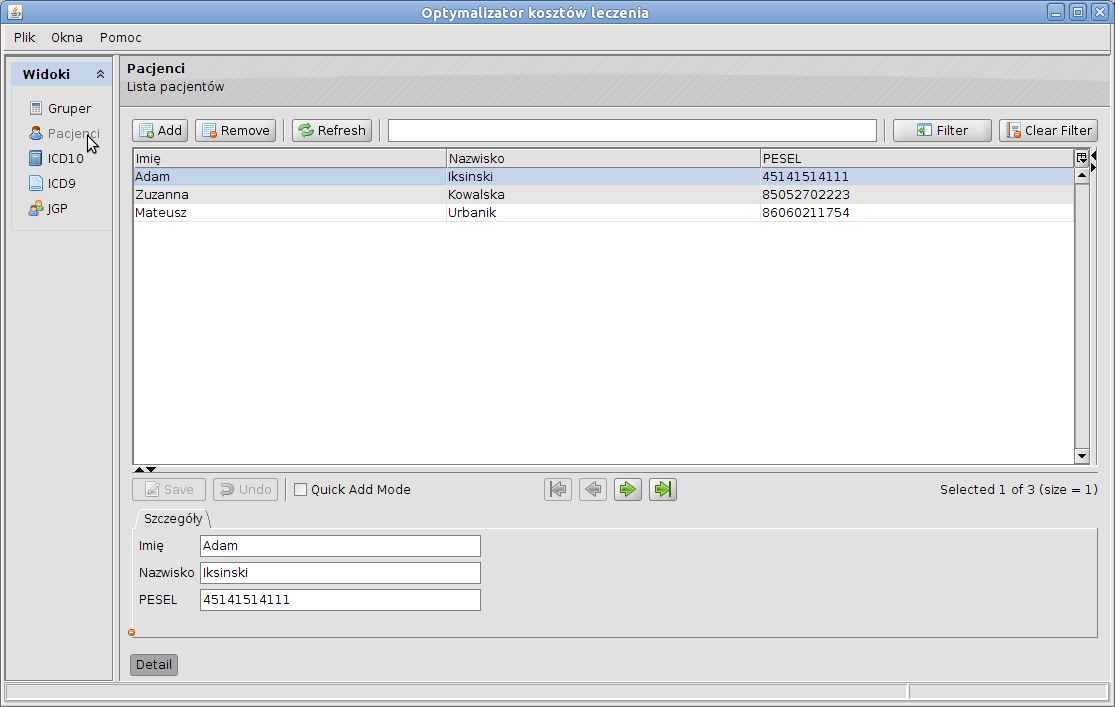
\includegraphics[scale=0.4]{images/patient} 

Na identycznym szablonie zbudowane są widoki: katalog kodów ICD-9, ICD-10, JGP. Z tą różnicą, że zablokowana jest możliwość dodawania, edycji i usuwania faktów z bazy wiedzy. Według założeń systemu ekspertowego może te operacje wykonywać tylko i wyłącznie inżynier wiedzy.

%---------------------------------------------------------------------------

\section{Praktyczne użycie systemu}
\label{sec:praktyczneUzycieSystemu}
Aby zilustrować działanie aplikacji przedstawię w tym podrozdziale konkretny i realny przypadek użycia aplikacji. Zostanie wykorzystany również mechanizm dzięki, któremu lekarz ma możliwość optymalizacji kosztów leczenia pacjenta.

Zdefiniujmy więc fakty wejściowe. Leczony pacjent urodzony w 1937 roku ma 75 lat, jest mężczyzną, przyjęty był na okres 7 dni w trybie przyjęcia ,,Przyjęcie planowe na podstawie skierowania'' oraz wypisany trybie ,,Zakończenie procesu terapeutycznego lub diagnostycznego''. Typ hospitalizacji: ,,Hospitalizacja zwykła''.

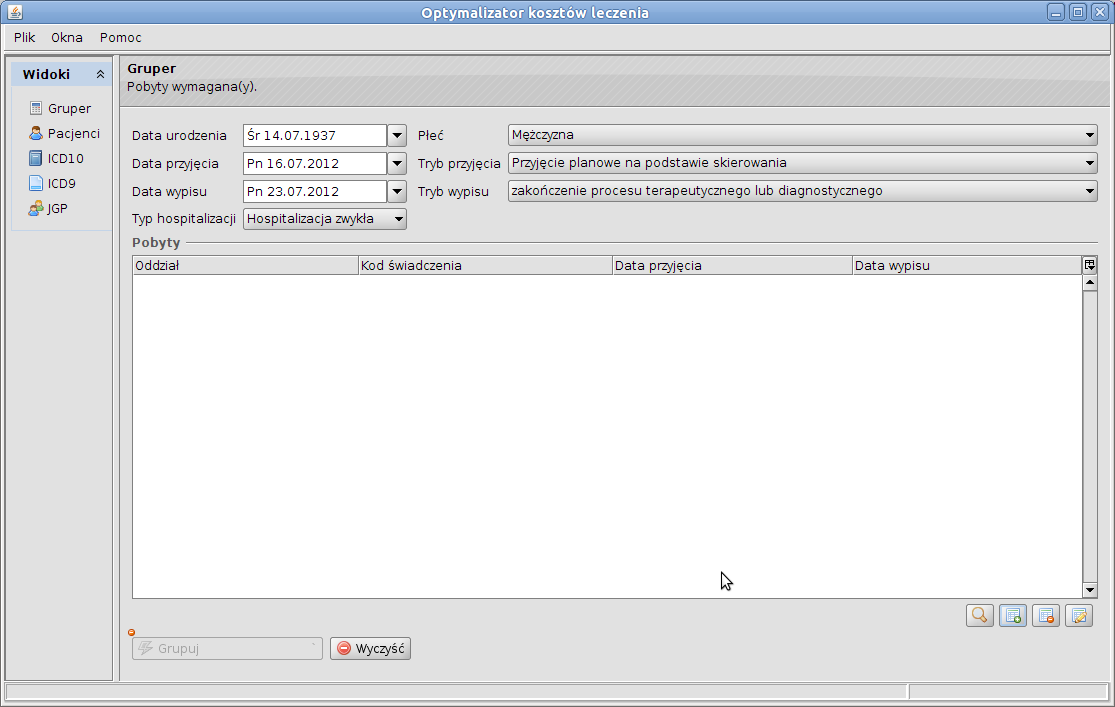
\includegraphics[scale=0.4]{images/gruper1}

Następnie należy zdefiniować pobyt. Ustalamy dane pobytu: odział kod świadczenia, data przyjęcia i wypisu przepisuje się auomatycznie.

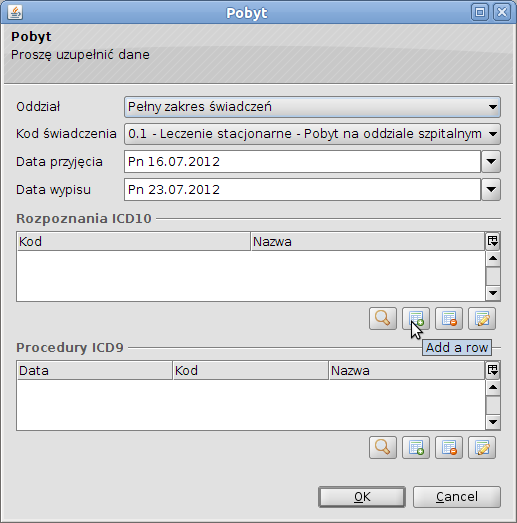
\includegraphics[scale=0.4]{images/gruper2}

Kolejnym krokiem jest dodanie zdiagnozowanych rozpoznań. U pacjenta stwierdzono:

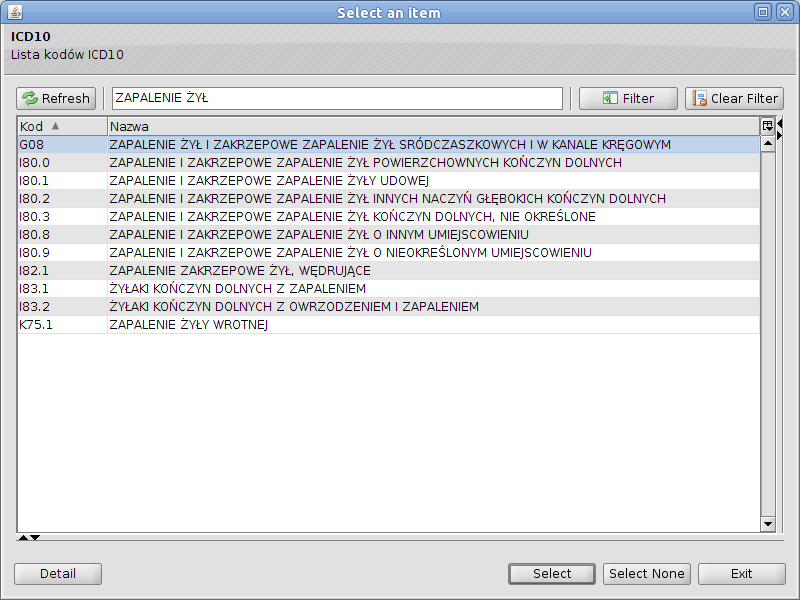
\includegraphics[scale=0.4]{images/gruper3}

Dodajemy rozpoznanie do pobytu klikając przycisk Select.

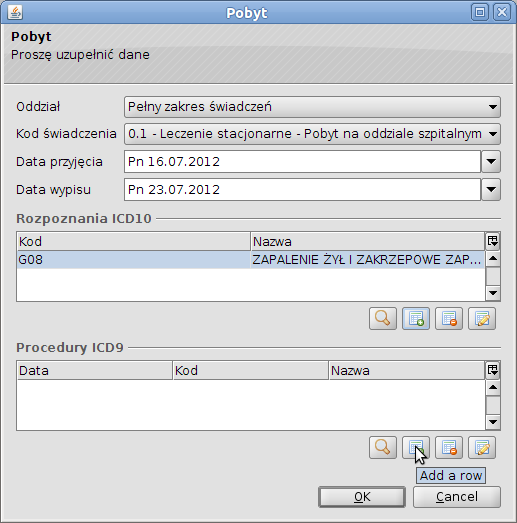
\includegraphics[scale=0.4]{images/gruper4}

Następnie dodajemy wykonane procedury medyczne, klikamy przycisk Dodaj procedurę.

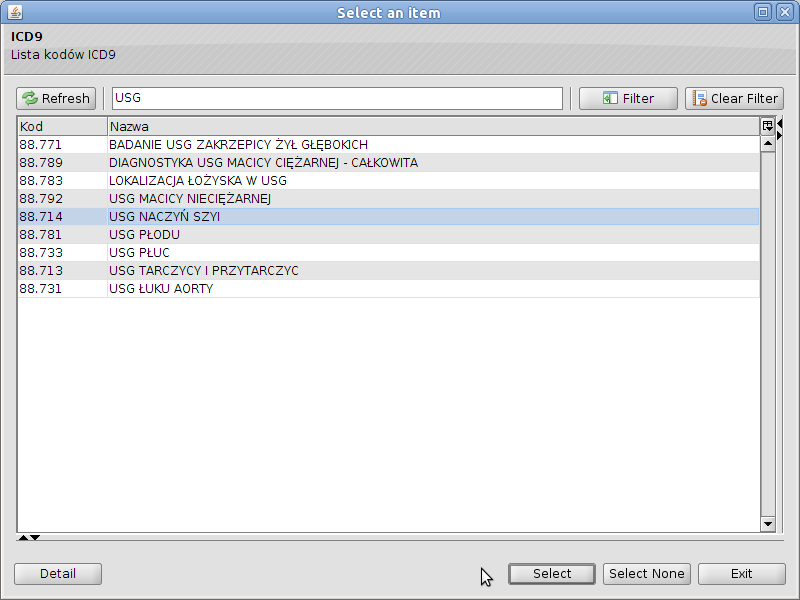
\includegraphics[scale=0.4]{images/gruper5}

Po wybraniu procedury musimy ustalić w jakim terminie została oan wykonana oraz ile razy.

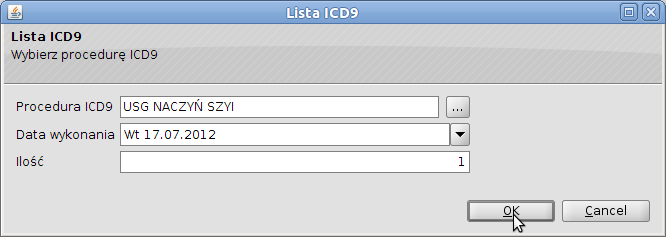
\includegraphics[scale=0.4]{images/gruper6}

Po kliknięciu OK, wracamy do okienka z prawidłowo zdefiniowanym pobytem.

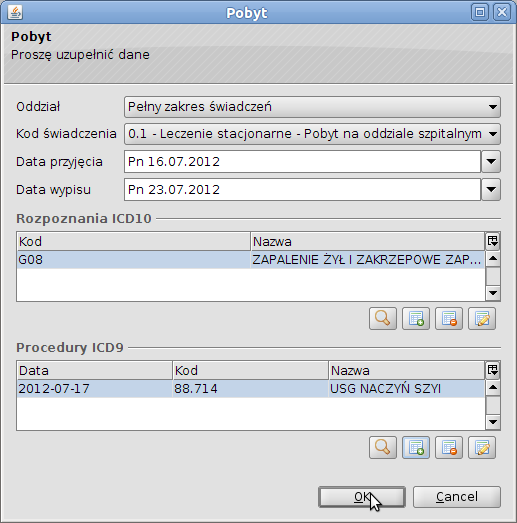
\includegraphics[scale=0.4]{images/gruper7}

Widok groupera z wypełnionymi wszystkimi danymi wejściowymi prawidłowo, pozwala na uruchomienie algorytmu użytkownikowi. Należy nacisnąć przycisk Grupuj.

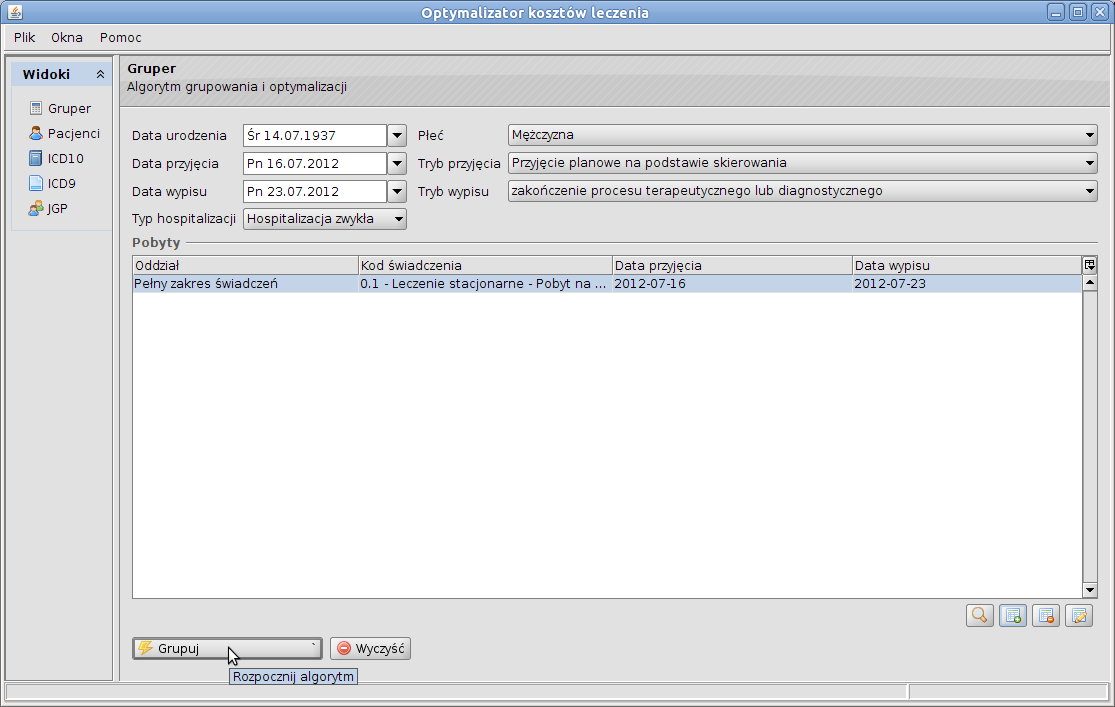
\includegraphics[scale=0.4]{images/gruper8}

Uruchamiany jest algorytm wnioskowania, który wybiera warunki do sprawdzenia, testuje je, a wyniki zapisuje na listach: Zaakceptowane, Potencjalnie droższe, Potencjalnie tańsze.

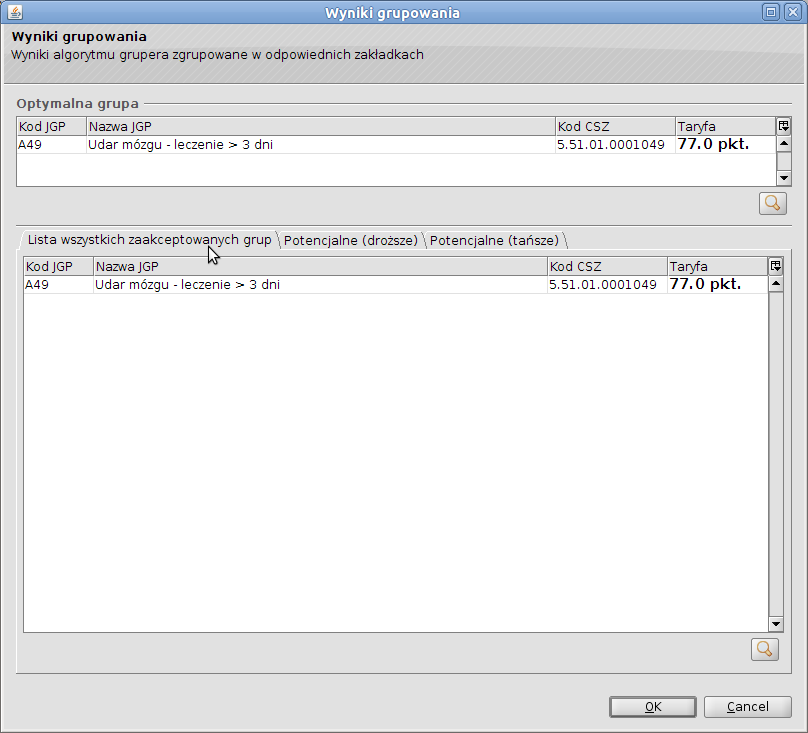
\includegraphics[scale=0.4]{images/gruper9}

W tym miejscu można zakończyć przebieg grupowania. Została wybrana optymalna grupa JGP: ,,A49 - Udar mózgu - leczenie > 3 dni'' oraz ustalona została wartość kosztów leczenia 77pkt.

Spróbujmy zoptymalizować koszty leczenia. Dla placówki, która często jest zadłużona na niebagatelne kwoty i jest na skraju bankructwa bardzo ważna jest maksymalizacja kosztów leczenia. Odpowiednie narzędzia pozwalające przewidywać wyliczane według NFZ koszty leczenia pacjenta może sprawić, że placówka ma możliwość wygenerowania większych zysków z wykonywanej pracy, a pacjent będzie leczony lepiej. Co należy zrobić, aby zmaksymalizować koszty leczenia dla naszego przypadku? Na tym etapie należy spojrzeć na zakładkę ,,Potencjalnie droższe''. Będą tam grupy JGP które będą nas właśnie szczególnie interesować.

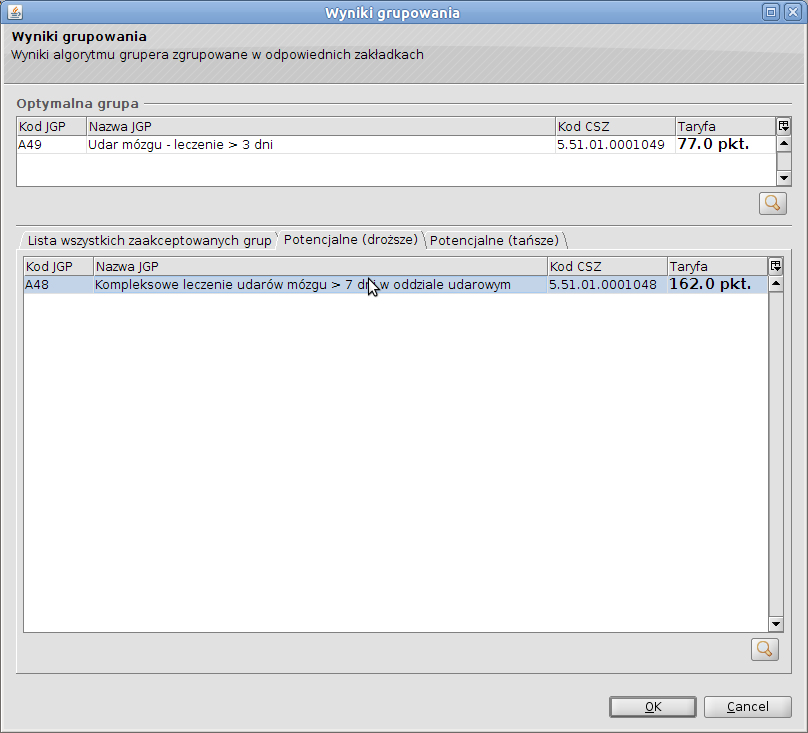
\includegraphics[scale=0.4]{images/gruper10}

Widać, że istnieje grupa JGP dająca możliwośc wygenerwoania kosztów w wysokości 162pkt. Jest to ponad 2-krotnie większa wartość od wyliczonej aktualnie! Co zrobić, żeby zakwalifikować leczenie do tej grupy systemu JGP. Klikamy w przycisk Szczegóły i patrzymy na powody niezaakceptowania grupy.

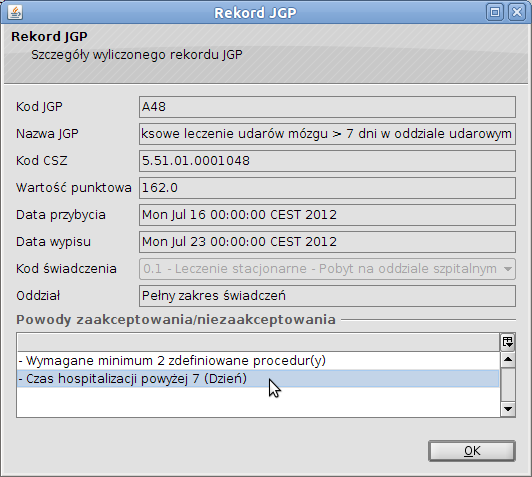
\includegraphics[scale=0.4]{images/gruper11}

Są dwa powody niezaakceptowania pacjenta:
- wymagane minimum 2 procedury
- czas hospitalizacji powyżej 7 dni.

W tym momencie zakres działania aplikacji się kończy, Jest to system doradczy, a decyzję optymalizacyjną podejmuje lekarz. Dla naszego przypadku leczenia lekarz stwierdza, że przetrzymanie pacjenta 1 dzień dłużej na oddziale i wykonanie dodatkowego badania podwoi koszty leczenia. I lekarz decyduje się na przedłużenie leczenia o 1 dzień.

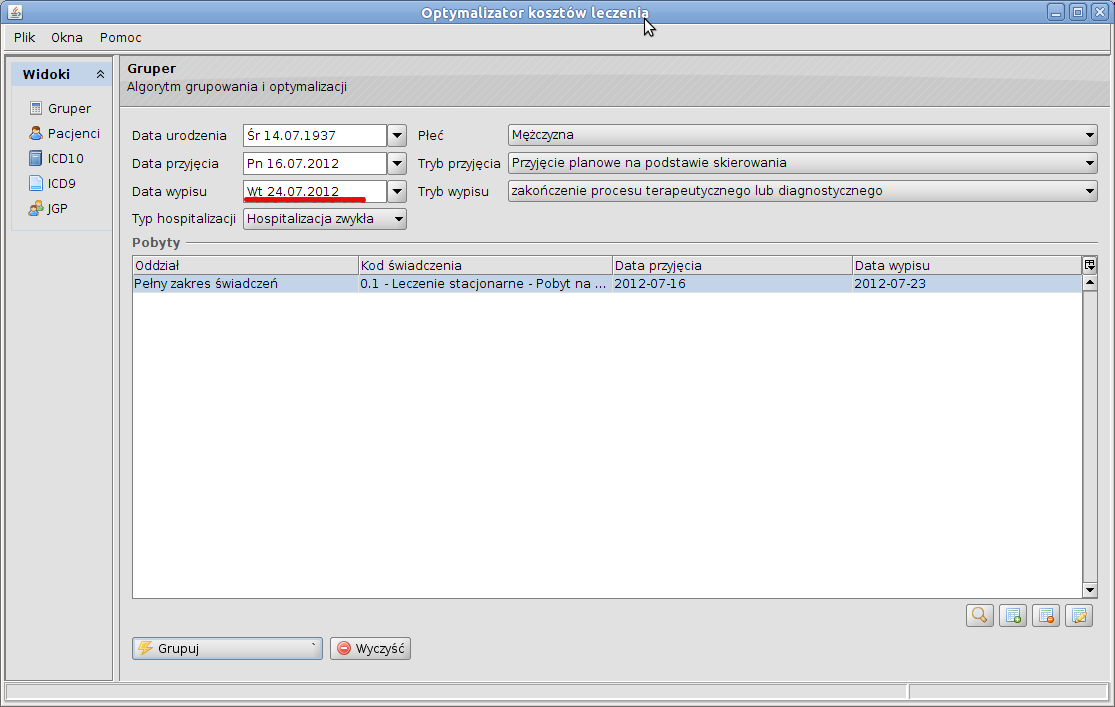
\includegraphics[scale=0.4]{images/gruper12}

I dodajemy kolejną procedurę medyczną, badanie radiologiczne: ,,Arteriografia tętnicy szyjnej wewnętrznej''.

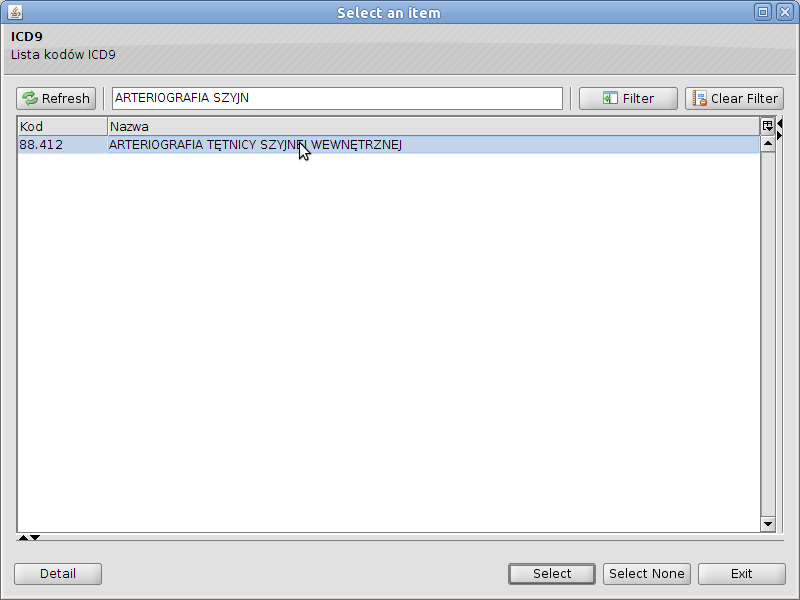
\includegraphics[scale=0.4]{images/gruper13}

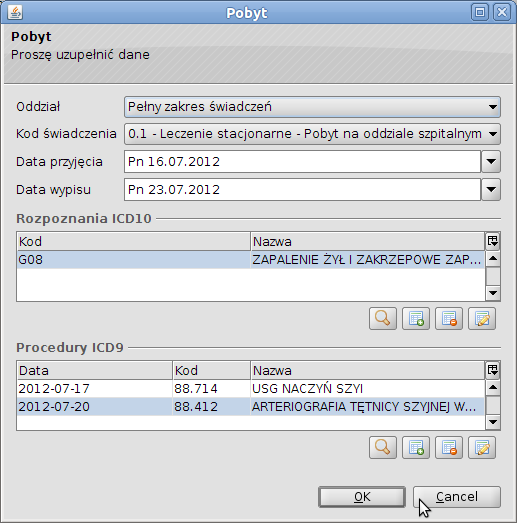
\includegraphics[scale=0.4]{images/gruper14}

W wyniku ponownego uruchomienia algorytmu grupowania, otrzymuje jako wynik zaakceptowaną i optymalną grupę JGP, na której na zależało:

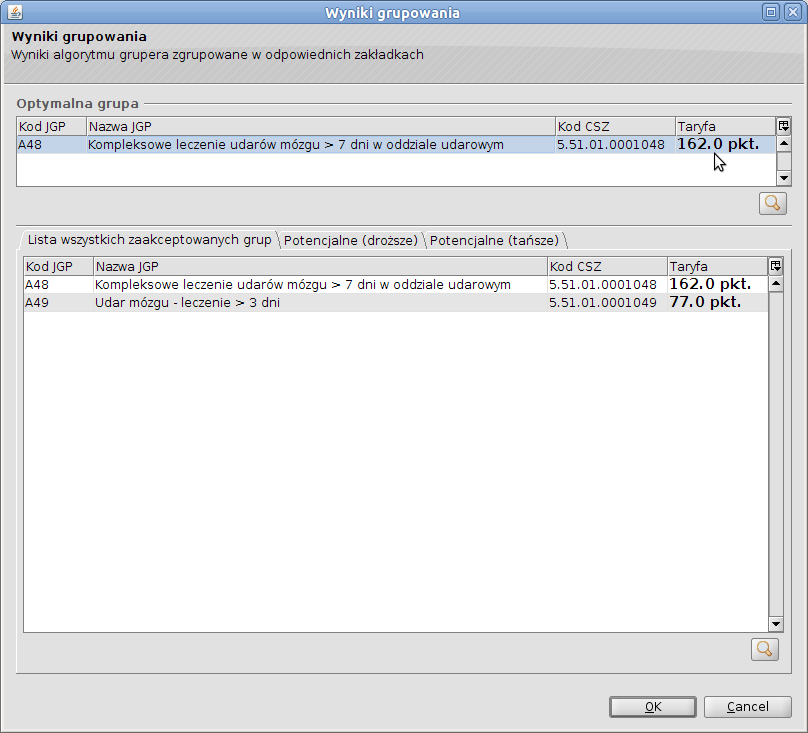
\includegraphics[scale=0.4]{images/gruper15}

Wybrana zostaje grupa A48 - Kompleksowe leczenie udarów mózgu > 7 dni w oddziale udarowym. Koszt leczenia to 162 jednostki punktowe.

%---------------------------------------------------------------------------

\section{Testy integracyjne}
\label{sec:testyIntegracyjne}

Takich przypadków użycia aplikacji jest na prawdę bardzo wiele. Aplikacje wysokiej jakości charakteryzują się wysokim pokryciem kodu w testach. Postanowiłem zatem napisać testy integracyjne klasy JGPService. Stworzyłem klasę JGPServiceTest, której zadaniem jest przetestowanie 26 przypadków użycia algorytmu grupowania, gdzie grupa wynikowa będzie pochodzić z konkretnego warunku kierunkowego. A wieć poszczególne testy są napisane w ten sposób, aby przetestować każdy z możliwych 26 warunków kierunkowcyh A-Z.
Przykład przedstawiony powyżej został również zaimplementwoany w testach. Jest to test sprawdzający poprawność działania warunku kierunkowego E - grupa zdefiniowana procedurą i rozpoznaniem zasadniczym; może mieć dodatkowe warunki (czas hospitalizacji, wiek).
Dla testów integracyjnych przygotowana jest baza wiedzy. Ustalane są dane epizodu, uruchamiany jest mechanizm wnioskowania. A następnie sprawdzane są wyniki. Testowana jest poprawność wyników z listy zaakceptowanych kodów oraz z listy niezaakceptowanych kodów, wraz z testami powodów niezaakceptowania.
Kod przykładowego testu integracyjnego:
\begin{verbatim}
@Test
public void testGrouperE() {
    Episode episode = createTestEpisode(new String[]{"G08"}, new String[]{"88.714"}, 7, 75);
    //run grouper
    JGPGroupResult result = jgpService.group(episode);
    //test accepted
    Assert.assertEquals(1, result.accepted().size());
    JGPResult acceptedJGP = result.accepted().get(0);
    Assert.assertEquals(77.0, acceptedJGP.getValue(), 0.0);
    Assert.assertEquals("A49", acceptedJGP.getJgp().getCode());
    //test NOT accepted
    Assert.assertEquals(1, result.notAccepted().size());
    JGPResult notAcceptedJGP = result.notAccepted().get(0);
    Assert.assertEquals(162.0, notAcceptedJGP.getValue(), 0.0);
    Assert.assertEquals("A48", notAcceptedJGP.getJgp().getCode());
    HospitalReason hospReason = notAcceptedJGP.reasons(HospitalReason.class).get(0);
    Assert.assertEquals(7, hospReason.required().getOver().intValue());
    Assert.assertEquals(TimeUnit.DAY, hospReason.required().getTimeUnit());
}
\end{verbatim}

